\chapter{Motion}
\label{motion}

% **************************** Define Graphics Path **************************
\graphicspath{{Chapter5/Figs/}}


\section{Introduction}
Contemporary computer vision models are extremely effective at understanding individual images. Given enough training data, deep convolutional neural network architectures can learn powerful representations using end-to-end supervised learning \cite{krizhevsky2012imagenet,he2016deep}. For scene understanding, models can extract rich information at a pixel level such as semantics \cite{long2015fully,badrinarayanan2017segnet,he2017maskrcnn} and geometry \cite{eigen2015predicting,garg2016unsupervised}.
However, there is a limit to what we can infer from static images. To effectively understand complex and dynamic scenes we need to reason over video.

Designing models which can learn motion and reason over temporal sequences is of critical importance for computer vision systems. Video and temporal information allows models to encode motion, reason over occlusions and improve temporal consistency and stability. Additionally, many scene understanding systems are required to inform decision making processes. Usually, these decision-making processes cannot be made in temporal isolation and, particularly in robotics, knowledge of scene dynamics is essential.

State of the art video scene understanding systems typically process individual frames independently \cite{he2017maskrcnn,zhao2017pspnet,eigen2015predicting,zhou2017unsupervised,patraucean2015spatio,valipour2017recurrent,gadde2017semantic}. Additional temporal reasoning can be performed by filtering \cite{miksik2013efficient} or with graphical models \cite{de2012line,chen2011temporally,tripathi2015semantic,hur2016joint}, however these systems are unable to be trained jointly and have significantly higher computational requirements. Many papers have proposed to add temporal components such as recurrent neural networks \cite{hochreiter1997long} on top of semantic segmentation encoders \cite{patraucean2015spatio,valipour2017recurrent}. However, to date, none have been able to demonstrate improvement over equivalent per-frame models at scale. In this paper, we observe the same result; naive sequence-to-sequence modelling from video with recurrent convolutional models harms semantic segmentation performance. We argue that this is because the recurrent units propagate their state from a static location in pixel space over time. However, in practice objects will move significantly in pixel location between consecutive frames due to camera ego-motion and scene dynamics. These models are not aware of this geometry and motion.

\begin{figure}[t]
\begin{center}
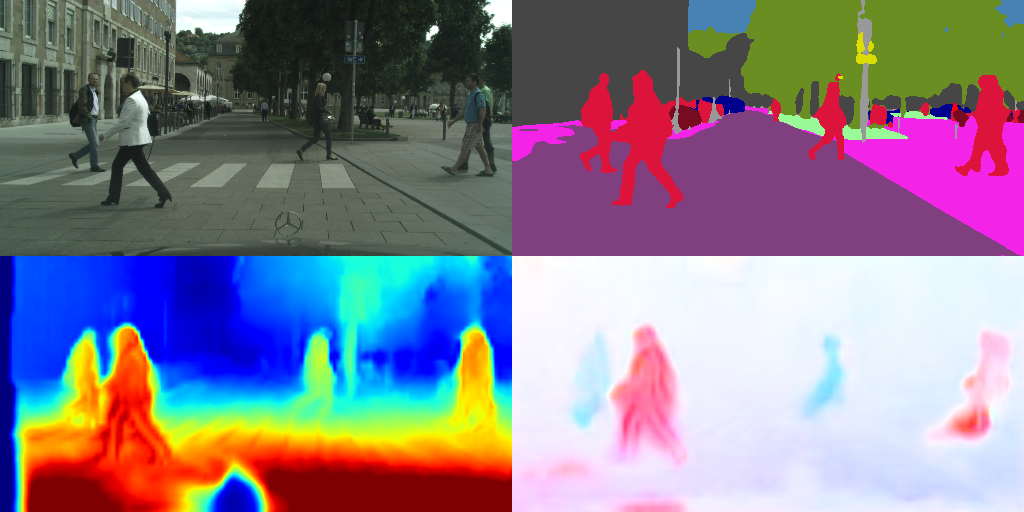
\includegraphics[width=0.7\columnwidth,trim={7mm 12mm 7mm 5mm},clip]{videosegnet.png}
\end{center}
   \vspace{-5mm}
   \caption[Video scene understanding.]{\textbf{Video scene understanding.} Our model jointly learns to estimate scene motion (bottom right), depth (bottom left) and semantic segmentation (top right), in addition to estimating ego-motion over video input. We learn semantics with supervised learning and are able to learn geometry and motion using self-supervised learning, without labelled training data.} % Code and video results can be found at the following website: \texttt{url released with publication}}
\label{fig:teaser}
   \vspace{-5mm}
\end{figure}

In this paper, we introduce an end-to-end deep learning architecture for video semantic segmentation. We jointly learn optical flow, ego-motion and depth with self-supervised learning and semantic segmentation with supervised learning. We propose a motion-aware gated recurrent unit (motion-GRU) which is able to use motion and geometry to account for ego-motion and scene dynamics when propagating state information temporally. Since labelling video frames with semantic labels is prohibitively expensive, we show that learning geometry with unsupervised learning can provide a powerful dense training signal for video. In summary, the novel contributions of this paper are;
\begin{enumerate}%[topsep=0.5ex,itemsep=0ex,partopsep=1ex,parsep=1ex]
\item showing how to account for motion when propagating recurrent states over time by using motion recurrent units,
\item demonstrating how to provide training signal for each video frame with self-supervised learning of motion and geometry,
\item using temporal augmentation of video data in order to learn a stable representation over time.
\end{enumerate}

In the remainder of this paper, we discuss these ideas and show how to train large temporal models over long video sequences at scale. We show that our model is able to perform video semantic segmentation with higher accuracy and temporal consistency than equivalent per-frame models.



\section{Video Scene Understanding} 

Scene understanding is the task of extracting information about the objects and their contextual relationships from the observed environment. Supervised deep learning is a very effective solution to this problem from single images. In particular, many deep convolutional encoder-decoder architectures have been shown to produce accurate and real-time solutions to problems such as semantic segmentation, optical flow, depth and geometry estimation.

Semantic segmentation is the task of estimating the semantic class of each pixel in an image. State of the art models use supervised deep learning \cite{badrinarayanan2017segnet,long2015fully}, benefiting from residual architectures \cite{he2016deep,huang2017densely}. Recent work has focused on improving the receptive field of features and providing them with more context for semantic reasoning, for example using dilated convolutions \cite{YuKoltun2016} and pyramid spatial pooling \cite{zhao2017pspnet}. We have also seen semantic segmentation combined with other tasks, such as instance segmentation \cite{he2017maskrcnn} and geometry \cite{kendall2017multi} in multi-task learning settings. Probabilistic modeling and Bayesian deep learning has also been used to understand model uncertainty in scene understanding algorithms \cite{kendall2017uncertainties,kendall2015bayesian}, improving safety in practical applications.

Depth and geometry models use similar architectures to semantic segmentation, but in a regression setting. Typically they estimate per-pixel metric depth or surface normals \cite{eigen2015predicting}. In \cite{UZUMIDB17} the authors learn geometry and motion using supervised learning. Deep learning models can also be trained using unsupervised learning without explicit depth labels using reprojection into stereo \cite{garg2016unsupervised} or temporal \cite{zhou2017unsupervised} frames. End-to-end deep learning can also be used to estimate depth from stereo vision \cite{kendall2017end}.

The problem of estimating motion in video is known as optical flow. Specifically, optical flow is a measurement of each pixel's 2D motion between subsequent video frames. It captures motion due to the ego-motion of the camera (which can be represented by the fundamental matrix for two frames \cite{hartley2003multiple}) and motion due to scene dynamics. State-of-the-art real-time models use deep learning \cite{flownet,flownet2} and are often trained on large synthetic datasets.

Video scene understanding, and video semantic segmentation, requires these tasks to be performed over video. Video and temporal information allows models to encode motion, reason about occlusion and improves temporal consistency and stability. Initial methods approached temporal modelling as a filtering problem \cite{miksik2013efficient}.
However, the most popular approach to date has been to construct large graphical models that connect different video pixels to achieve temporal consistency across frames \cite{de2012line,chen2011temporally,tripathi2015semantic,hur2016joint}. For example,\cite{chen2011temporally} used dynamic temporal links between the frames but optimized for a 2D CRF with temporal energy terms.
A 3D dense CRF across video frames is constructed in \cite{tripathi2015semantic} and optimized using mean-field approximate inference. In \cite{hur2016joint} a joint model to infer flow and semantic segmentation was proposed.

Geometry, in the form of structure from motion, has been used to aid video segmentation with random forests \cite{brostow2008segmentation} and Markov random fields \cite{tighe2013superparsing}.
More recent works look at jointly modelling 2D semantics and 3D reconstruction of scenes from video \cite{kundu2014joint,sengupta2013urban}.

Deep learning approaches for understanding video have been largely constrained to video level understanding tasks. For example, 3D convolutions have been used for off-line video classification \cite{karpathy2014large} or activity recognition \cite{ji20133d}. Additionally, LSTMs have been used for video recognition and captioning \cite{donahue2015long}. However these tasks require representations at a video level, and do not need to consider scene geometry and dynamics like in this work.

Single image semantic segmentation systems have also been adapted to video segmentation. For example, \cite{zhu2017deep,gadde2017semantic} both learn a representation warping module to form a two-frame video segmentation model. \textit{Clockwork} convolutional networks \cite{shelhamer2016clockwork} and \cite{zhu2017deep} both propose a way of reducing computation for video segmentation by reusing representations from single images across time.

To date, there have been a few proposals for video segmentation models over long video sequences with deep learning \cite{patraucean2015spatio,valipour2017recurrent}. They typically append a RNN or LSTM layer after a convolutional encoder-decoder model. However, so far every model has decreased model performance, compared to single frame non-video baseline models \cite{patraucean2015spatio,valipour2017recurrent}. We believe this work is the first to demonstrate an improvement in performance using end-to-end deep learning over many-frame video sequences.

Video segmentation has also been considered in an off-line setting. This is a very different problem setting to what we consider in this paper, as algorithms have access to future video frames, and are not constrained to real-time inference. For example, these methods can afford to use computationally expensive spatial-temporal CRFs \cite{kundu2016feature}. In computer graphics and animation this is known as rotoscoping \cite{miksik2017roam}. Other related works of note are future video frame prediction \cite{luc2017predicting} and label propagation \cite{budvytis2010label}.

Other related work is in video object segmentation and video motion segmentation. These works are largely driven by datasets like DAVIS \cite{Perazzi2016}. This problem focuses on segmenting a single object, or moving objects \cite{tsai2016video,tokmakov2017learning,vertens2017smsnet} in video. Unlike our work, explicit knowledge of semantics is not required. Rather, algorithms commonly use one-shot learning for masks and propagate them through video \cite{voigtlaender17BMVC}. Similar to scene understanding, the best approaches today segment single frames independently \cite{caelles2017one,khoreva2016learning}.

\section{Temporal Scene Understanding Model}
\label{sec:model}

\begin{figure*}[!t]
\begin{center}
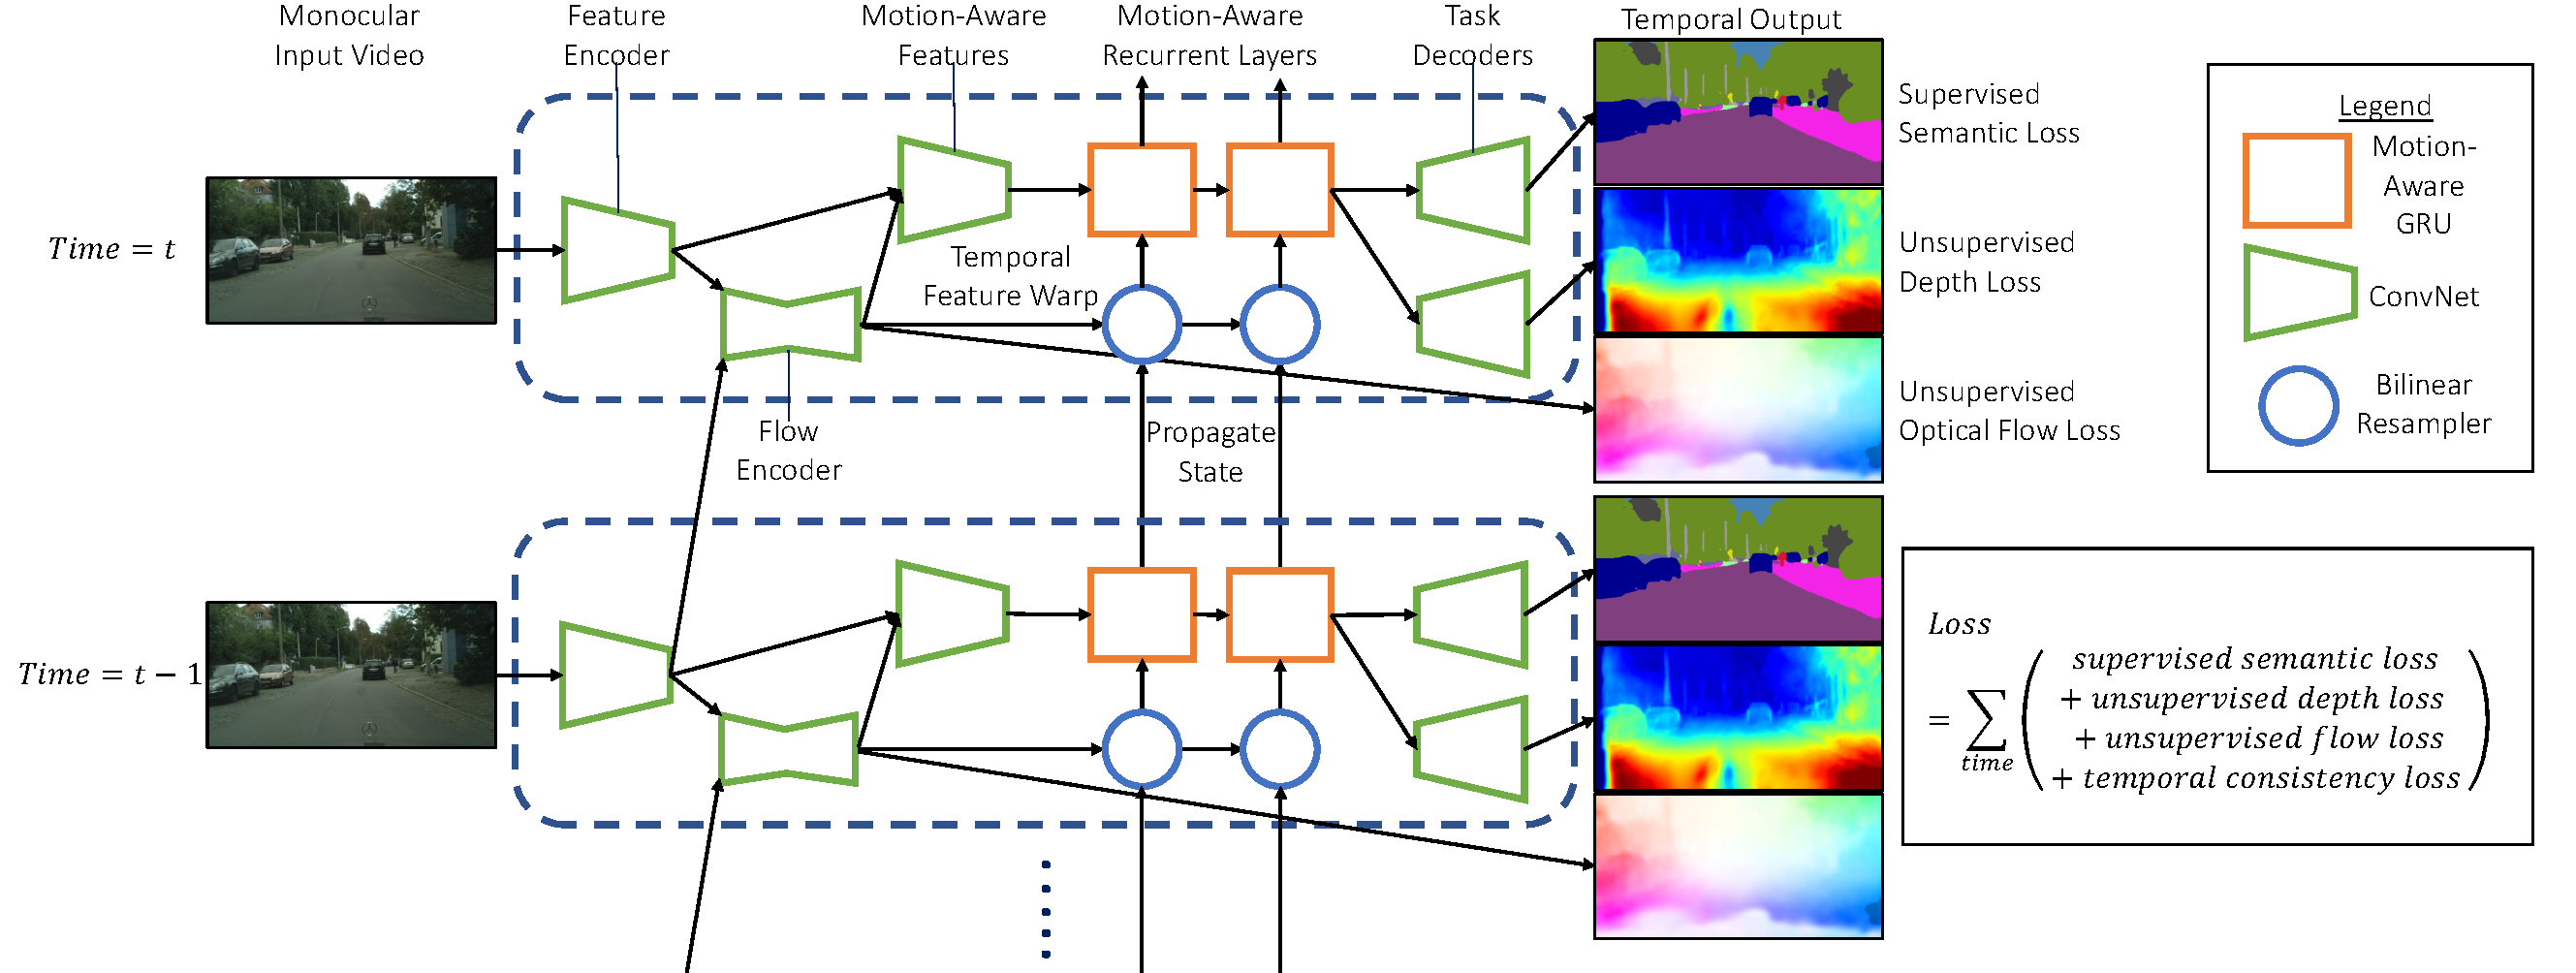
\includegraphics[width=\linewidth]{temporal_model.pdf}
\end{center}
\vspace{-5mm}
   \caption[Video scene understanding architecture.]{\textbf{Overview of our video scene understanding architecture.} The model efficiently propagates information over time, outputting semantic segmentation, depth, ego-motion and optical flow estimates from monocular video.}
\label{fig:arch}
\vspace{-2mm}
\end{figure*}

In this section we describe our model for video scene understanding, motion-aware recurrent neural network and the video loss functions.

\subsection{Architecture}

Consider a sequence of images, $I_0, I_1, ... , I_t$. We wish to produce a representation of the scene's semantics, motion and geometry in real-time for time-step, $t$.
In order to reduce the high dimensionality of the input, we pass the image through a deep convolutional encoder to obtain a powerful feature representation,
\begin{equation}
\mathbf{x}_t = encoder(I_t).
\end{equation}
We choose to use the E-Net architecture for our encoder \cite{paszke2016enet} because it achieves good segmentation performance while being computationally light-weight.

Using the feature representations from the previous and current time steps, we can then learn to regress optical flow (the motion of features between frames). We feed both these features through a network inspired by FlowNet simple \cite{flownet}:
\begin{equation}
\mathbf{y}^{flow}_{(t-1) \to t} = flownet(\mathbf{x}_t, \mathbf{x}_{(t-1)}).
\end{equation}
This results in an estimate of optical flow for each feature from the encoder, $\mathbf{y}^{flow}_{(t-1) \to t} $. We save computation by estimating flow using features shared by the semantic encoder, rather than the raw image. This is because initial filters in flow and semantic encoders will be very similar \cite{zeiler2014visualizing}. We also improve the representation by leveraging multi-task learning \cite{caruana1998multitask}.

In order to improve the feature representation for the current frame, and to incorporate motion, we concatenate the flow feature map (from the layer immediately prior to the flow regression), $\mathbf{y}'^{flow}_{(t-1) \to t}$, and the image features at the current time $\mathbf{x}_t$. We pass these features through some convolutional layers to learn a representation with motion-aware features:
\begin{equation}
\mathbf{z}_t = features(\mathbf{x}_t, \mathbf{y}'^{flow}_{(t-1) \to t})
\end{equation}
We implement $features$ as two residual layers \cite{he2016deep} with feature size $64$.

This results in a set of features, $\mathbf{z}_t$, at each time-step which encode image semantics and first order motion. Note that these features only have access to input signal from time $t$ and $t-1$. We now would like to learn long term dynamics over a sequence, to model higher-order motion and improve temporal consistency. A common approach to sequence modelling is to use a recurrent neural network (RNN). RNNs use an internal state to propagate memory over sequences. In particular, long-short-term-memory (LSTMs) units \cite{hochreiter1997long} have been shown to more effectively learn long dependencies. Gated recurrent units (GRU) \cite{cho2014learning} are a variant of LSTMs which retain the gated structure, but have a simpler internal structure making them faster to train.

Many papers have tried to place recurrent modules over features from a convolutional encoder \cite{patraucean2015spatio,valipour2017recurrent}. However, every attempt has not improved over per-frame baseline models. We make the observation that each recurrent module propagates its state forward in time for each spatial location in its feature map. However, objects in the scene rarely remain in the same location in pixel coordinates across video frames. This is due to the dynamic nature of real world environments, and ego-motion of the camera. This poses a problem for the recurrent state. This is because the state at time $t-1$, for a given pixel coordinate $(u,v)$, is unlikely to contain information about the same object which likely moved to a new pixel coordinate $(u',v')$ at the next time-step, $t$. Our hypothesis is that the propagation of misaligned features over time causes this decrease in performance with temporal models.

We propose to solve this problem by introducing a motion-aware GRU module. We know the motion of each pixel from our estimate of the optical flow, $\mathbf{y}^{flow}_{(t-1) \to t}$. Therefore we can align features over time, such that they account for motion of the object in pixel space, by warping the recurrent state and features using the estimate of optical flow. The full equations of our motion-aware GRU are;
\begin{align}
\mathbf{g}_t &= \text{sigmoid}(W_g * \mathbf{z}_t + U_g * \mathbf{h}^{warped}_{t-1} + b_g) \\
\mathbf{r}_t &= \text{sigmoid}(W_r * \mathbf{z}_t + U_r * \mathbf{h}^{warped}_{t-1} + b_r) \\
\mathbf{\widetilde{h}_t} &= \tanh (W_h * \mathbf{z}_t + U_h * \mathbf{r}_t \cdot \mathbf{h}^{warped}_{t-1}) \\
\mathbf{h}_t &= (1-\mathbf{g}_t) \cdot \mathbf{h}^{warped}_{t-1} + \mathbf{g}_t \cdot \mathbf{\widetilde{h}}_t,
\end{align}
with convolutional weights, $W, U$, and biases, $b$. We use a convolutional kernel size of 3 and add batch-normalisation after each convolution, which we omit for clarity. To form a motion-GRU, our model is going to use its estimate of optical flow to propagate the features temporally over the video sequence, such that the features correspond in pixel space. We do this by resampling features according to the optical flow map using bilinear interpolation, inspired by spatial transformer networks (STNs) \cite{jaderberg2015spatial}.
We define this function which warps the recurrent state, $\mathbf{h}_{(t-1)}$, from time $t-1$ to time $t$, by resampling using the optical flow vectors, $\mathbf{y}^{flow}_{(t-1) \to t}$, as follows:
\begin{equation}
\mathbf{h}^{warped}_{t} = warp(\mathbf{h}_{(t-1)}, \mathbf{y}^{flow}_{(t-1) \to t}).
\end{equation}
The motion-GRU then uses $\mathbf{h}^{warped}_{t}$ rather than $\mathbf{h}_t$ as input. We backpropagate gradients smoothly by implementing this warping with bilinear interpolation \cite{jaderberg2015spatial}. We can stack multiple GRU layers in series to model long term temporal information. Note, we can also form motion-RNNs and motion-LSTMs with the same change. We choose GRUs because of their ability to gate inputs and simple implementation.

Warping the state vectors between time-steps attempts to align features with their correspondences. However, due to occlusion, it is not possible to achieve this completely, as some features will appear and disappear with motion. We rely on the model to learn to understand this phenomena.

Finally, we learn separate decoders to estimate pixel-wise semantic segmentation and depth regression from the output of the motion-aware GRUs, $\mathbf{h}_t$.
\begin{align}
\mathbf{y}^{class}_t &= decoder_{class}(\mathbf{h}_t), \\
\mathbf{y}^{depth}_t &= decoder_{depth}(\mathbf{h}_t), \\
\mathbf{y}^{egomotion}_t &= decoder_{egomotion}(\mathbf{h}_t),
\end{align}
where class and depth decoders are comprised of a single $3\times 3$ convolutional layer with feature size 32 followed by a $1 \times 1$ convolutional layer regressing the required output dimensions ($1$ for depth and number of semantic classes for class). The ego-motion decoder uses global average pooling to pool the features, followed by a fully connected layer with feature size 32 and a final fully connected layer regressing a 6-DoF ego-pose vector, similar to \cite{zhou2017unsupervised}.

All layers are followed by batch normalisation and ReLU non-linearities, except for the prediction layers. For the depth prediction layer, we constrain the output to a reasonable positive range with $1/(\alpha * sigmoid (x) + \beta)$, with $\alpha = 0.99$ and $\beta = 0.01$ to constrain the depth values to reasonable limits.

This model can be run continuously over video in real-time to estimate per-frame optical flow, depth and semantic segmentation. This model is efficient and real-time because each image is only encoded once, and recurrent states are propagated through time. It is motion-aware from the two-frame optical flow feature input, which provides first-order motion information, and temporally aligns features. The recurrent state memory allows the model to remember higher order motion and reason over multiple views and deal with occlusion.

\subsection{Loss Function}

In this section, we explain how to learn semantic segmentation using supervised learning and optical flow, ego-motion and depth with self-supervised learning\footnote{We refer to this as self-supervised learning because we train the model with a regression target using our knowledge of geometry, in the absence of human-annotated labels. However, this has also been referred to as \textit{unsupervised learning} \cite{garg2016unsupervised,monodepth17,zhou2017unsupervised} or \textit{natural supervision} \cite{koltun2017natural} because of the lack of labels and the inability to evaluate the performance of the model against the data.}. The geometric outputs can be considered as intermediate auxiliary outputs. They assist learning semantic segmentation by making our model motion and geometry aware, improving the representation.

Large semantic segmentation datasets are available with thousands of densely labelled images \cite{lin2014microsoft,Cordts2016Cityscapes}.
Obtaining accurate depth and flow labels is much harder. Therefore, we use a self-supervised learning regime to learn flow and depth, based on the photometric reprojection error and multi-view geometry. We can learn depth by learning correspondence to stereo images \cite{garg2016unsupervised} or subsequent temporal frames \cite{zhou2017unsupervised}. We can learn flow by learning correspondences between temporal frames.

One possibility to learn depth is to use the estimated disparities, $\mathbf{y}_{depth}$, from input image, $I_t$, to warp the corresponding stereo image, $I_{t,stereo}$. We train on the photometric reconstruction error to form a loss function for depth estimation:
\begin{align}
\begin{split}
\mathcal{L}_{stereo~depth,~t} =& \frac{1}{N} \sum_{i,j} | I_t(i,j) - I_{t,stereo}(i,j+\mathbf{y}_{depth,t}(i,j)) |,
\end{split}
\label{eqn:depth}
\end{align}
where indices $i$ and $j$ correspond to pixel locations in the image. The loss is averaged across all temporal frames and pixels, $N$. Resampling pixel indices is performed by bilinear interpolation \cite{jaderberg2015spatial}. Minimising this loss causes the model to learn disparity. We omit the conversion from disparity to metric depth for clarity.

Alternatively, if stereo imagery is not avaliable, we can learn depth and ego-motion from monocular video \cite{zhou2017unsupervised}. We assume the camera's intrinsic matrix, $K$, is known. To estimate pixel correspondences in monocular video, we first back-project each homogeneous pixel coordinate, $p_{ijt}$, using the predicted depth:
\begin{align}
\begin{split}
X =  \mathbf{y}_{depth,t}(p_{ijt}) K^{-1} p_{ijt}.
\end{split}
\end{align}
We then transform these coordinates with the predicted ego-motion camera transformation from the current frame to the previous frame using the pose vector, $\hat{y}_t^{pose}$ which is represented as a $3\times4$ projection matrix, $\hat{T}_{t \to (t-1)}$,
\begin{align}
\begin{split}
\hat{p}_{ij(t-1)} = K \hat{T}_{t \to (t-1)} X.
\end{split}
\end{align}
We use these coordinates to resample $I_{t-1}$ and train on the photometric loss:
\begin{align}
\vspace{-1mm}
\begin{split}
\mathcal{L}_{mono~depth,~t} =& \frac{1}{N} \sum_{i,j} | I_t(p_{ijt}) - I_{(t-1)}(\hat{p}_{ij(t-1)}) |,
\end{split}
\label{eqn:monodepth}
\end{align}
to learn geometry from monocular video. Although, this only allows us to estimate depth and ego-motion up to some unknown scale-factor.

% PAMI: add explaination in detail of bilinear warping!!

To learn optical flow, we can warp the previous frame to the current frame, except now our disparity estimates have two-degrees of freedom to represent optical flow. Again, the loss is formed using the temporal, photometric reconstruction error:
\begin{align}
\begin{split}
\mathcal{L}_{flow,~t} = \frac{1}{N} \sum_{i,j}& | I_t(i,j) - I_{(t-1)}(i+\mathbf{y}_{flow~i,t}(i,j),j+\mathbf{y}_{flow~j,t}(i,j))) |.
\label{eqn:flow}
\end{split}
\end{align}
In \eqn{depth}, \eqn{monodepth} and \eqn{flow} the photometric reprojection error function is non-informative in homogeneous regions of the scene -- referred to as the aperture problem \cite{hartley2003multiple}. For example, in repetitive or texture-less surfaces, multiple disparities can generate equally good losses. Only when considering wider context can we reason about these regions with sufficient information. For this reason, a prior is often applied to the loss function, typically a smoothing function, to overcome the aperture problem. Previous literature uses some form of the total variation (TV) loss \cite{rudin1992nonlinear} and minimises the norm of the gradients for the predicted depth maps \cite{garg2016unsupervised,zhou2017unsupervised}. In this work we regularise the output of both flow and depth estimates with the $L_1$ norm of the second order gradients:
\begin{align}
\begin{split}
\mathcal{L}_{smooth,~t} =& \frac{\lambda}{N} \sum_{i,j}  | \nabla^2 \mathbf{y}_{depth,t} | + | \nabla^2 \mathbf{y}_{flow,t} |,
\end{split}
\label{eqn:smoothing}
\end{align}
Following \cite{zhou2017unsupervised}, we use the weighting factor of $\lambda = 0.5$.

We learn semantic segmentation with the cross entropy loss between semantic segmentation prediction and ground truth label for all semantic classes, $c$.
Typically, frames in video sequences are only sparsely labeled \cite{Cordts2016Cityscapes}. We therefore average the loss across only pixels and frames with ground truth labels, ignoring all others.
However, cross entropy treats each pixel independently in space and time. Additionally, we would like to encourage the network to learn a temporally consistent solution. We define a temporal consistency loss, which penalises temporal differences in segmentation prediction, after accounting for motion using optical flow:
\begin{multline}
\vspace{-1mm}
\mathcal{L}_{consist,~t} = \frac{1}{N} \sum_{i,j} | \mathbf{y}_{class,t}(i,j) - \mathbf{y}_{class,(t-1)}(i+\mathbf{y}_{flow~i,t}(i,j),j+\mathbf{y}_{flow~j,t}(i,j)) |,
\label{eqn:consistency}
\vspace{-3mm}
\end{multline}
where $\mathbf{y}(i,j)$ represents the semantic logit at pixel location $i,j$. The intuition here is that, if the optical flow estimate is correct, then corresponding pixel locations should represent the same semantic class.

The total loss combines the individual losses: depth \eqn{depth}, flow \eqn{flow}, classification and consistency \eqn{consistency}.We average the loss over all timesteps. Because we are optimising multiple losses, this is a multi-task learning problem \cite{caruana1998multitask}. A naive choice of overall loss would be to sum each individual loss:
\begin{equation}
\mathcal{L}_{total} =\frac{1}{T} \sum_{t=0}^T  \mathcal{L}_{class,t} +\mathcal{L}_{flow,t} +\mathcal{L}_{depth,t} +\mathcal{L}_{smooth,t} +\mathcal{L}_{consist,t} .
\end{equation}
However, Kendall et al. \cite{kendall2017multi} showed that the choice of weights between the losses in deep learning models has a very strong effect on overall performance. They propose a method to learn these weights automatically by considering each task's uncertainty. We use this method to automatically weight the losses as proposed in \cite{kendall2017multi}:
\begin{equation}
\vspace{-1mm}
\mathcal{L} = \sum_{\mathcal{L}_i \in [\mathcal{L}_{0}, \mathcal{L}_{1}, ..., \mathcal{L}_{N}]} \frac{1}{2 \sigma_i^2} \mathcal{L}_i + \log \sigma_i,
\label{eqn:multitask}
\vspace{-1mm}
\end{equation}
where we estimate the task (homoscedastic) uncertainty of each loss, $i$, by optimising a variable, $\sigma_i$. We \textit{do not} learn a weight for the consistency and smoothing regularisation losses. This formulation decreases the weight for tasks which have higher variance in their residuals. This is important because we are learning outputs with many different units: semantics as probability distributions, depth as a distance and optical flow in pixels. This formulation is able to balance the losses and learn a representation which is effective for each task: flow, depth and semantic segmentation.



\section{Experiments}

In this section we perform a number of experiments to evaluate the importance of compensating for motion in our architecture in addition to other design decisions. All experiments include all features of the model described in \sct{model}, unless otherwise stated. By default we train over four time-steps, with a warm-up of four steps. The entire model is randomly initialised before training.

\textbf{Dataset.} We use the CityScapes dataset for all experiments \cite{Cordts2016Cityscapes} which is a road scene understanding dataset. The CityScapes dataset was taken from a vehicle in various locations around Germany. It provides $5000$ stereo images with $1024 \times 2048$ resolution (of which $2,975$ are for training) with dense semantic segmentation labels. It also provides $19$ preceding and $10$ future frames around each labelled frame.
%In some experiments, we also make use of the propagated CityScapes dataset \cite{budvytis2017large}. 
In order to train our video model in GPU memory over long sequences, we sub-sample CityScapes images by a factor of two, to $1024\times 512$ resolution for training and testing. The original E-Net, which we use as our encoder, is also trained on this resolution.

The CityScapes dataset provides disparity labels from a stereo algorithm \cite{Cordts2016Cityscapes} which we use as pseudo-ground truth to compute depth error metrics. We measure depth error in disparity, converting from depth using the provided CityScapes stereo baseline. We use the output of FlowNet 2.0 \cite{ilg2017flownet} as a reference measure of optical flow, and the output of ORB-SLAM \cite{mur2015orb} for ego-motion, in order to evaluate our self-supervised predictions. We evaluate ego-motion with absolute trajectory error over a 5-frame sequence.

\textbf{Metrics.} We evaluate semantic segmentation performance with three metrics. First, mean intersection over union (IoU) measures the pixel wise semantic performance. It penalises false negatives and false positives. We also evaluate the \textit{temporal consistency} (TC) of the predicted semantic labels to measure if our video model produces more consistent and coherent results. We define temporal consistency as the percentage of pixels along an optical flow track which have the same class prediction. We evaluate depth metrics using inverse depth error in pixel disparity, scaled by the stereo baseline. We evaluate optical flow metrics in pixels and ego-motion error in meters.

\textbf{Optimisation.} For all experiments, we use a batch size of sixteen on a machine with four NVIDIA Titan Xp GPUs. We train with stochastic gradient descent, with $0.9$ momentum and a base learning rate of 0.1. We decay this learning rate using a polynomial schedule defined by \cite{chen14semantic} over $100,000$ training iterations. With these learning hyper-parameters our per-frame baseline of E-Net significantly outperforms the author's original implementation of the architecture \cite{paszke2016enet}.

\begin{figure*}[t]
\begin{subfigure}[t]{\linewidth}
\begin{center}
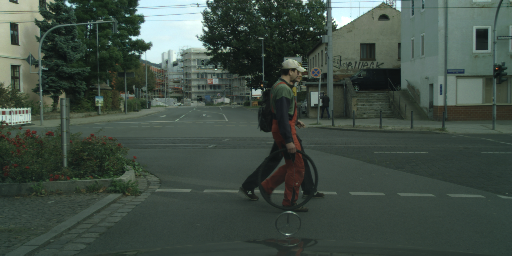
\includegraphics[width=0.19\linewidth]{image_000050_000019_image.png}
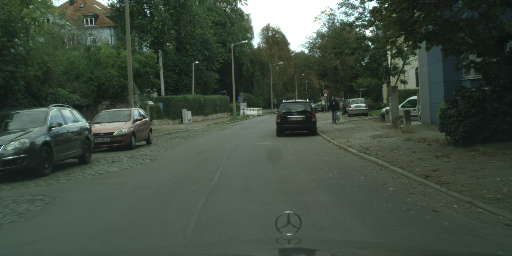
\includegraphics[width=0.19\linewidth]{image_000045_000019_image.png}
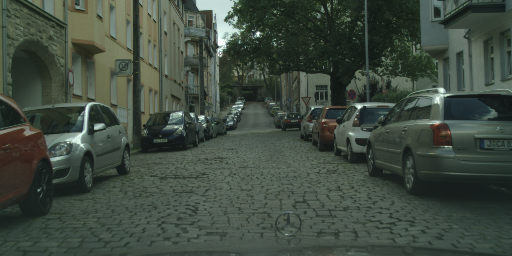
\includegraphics[width=0.19\linewidth]{image_000046_000019_image.png}
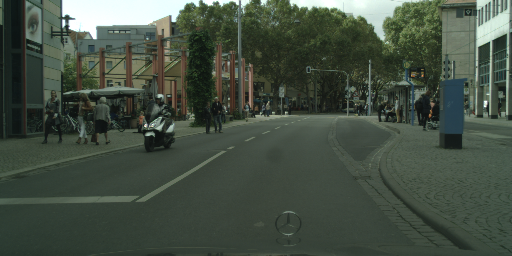
\includegraphics[width=0.19\linewidth]{image_000038_000019_image.png}
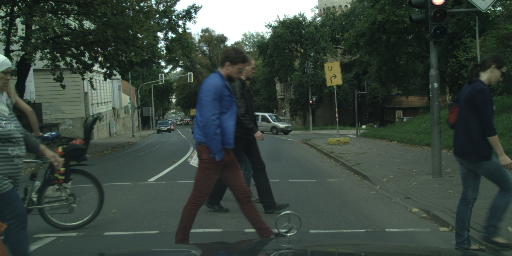
\includegraphics[width=0.19\linewidth]{image_000071_000019_image.png}
\vspace{-2mm}
  \caption{Input test images from video}
\end{center}
\end{subfigure}

\begin{subfigure}[t]{\linewidth}
\begin{center}
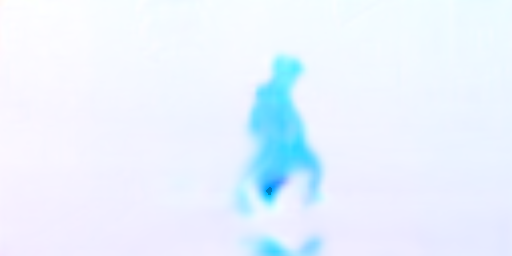
\includegraphics[width=0.19\linewidth]{image_000050_000019_flow.png}
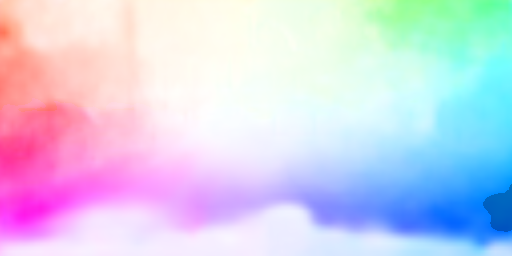
\includegraphics[width=0.19\linewidth]{image_000045_000019_flow.png}
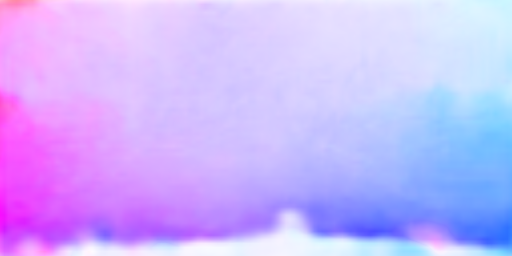
\includegraphics[width=0.19\linewidth]{image_000046_000019_flow.png}
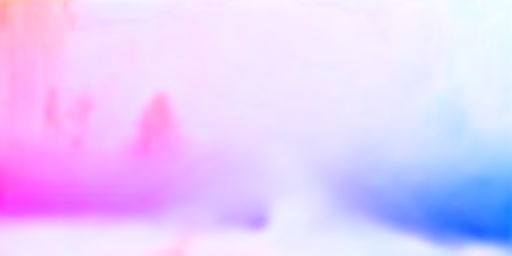
\includegraphics[width=0.19\linewidth]{image_000038_000019_flow.png}
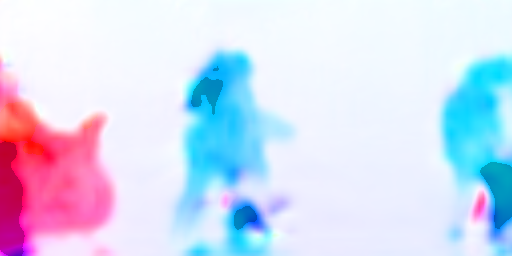
\includegraphics[width=0.19\linewidth]{image_000071_000019_flow.png}
\vspace{-2mm}
  \caption{Optical flow estimation}
\end{center}
\end{subfigure}

\begin{subfigure}[t]{\linewidth}
\begin{center}
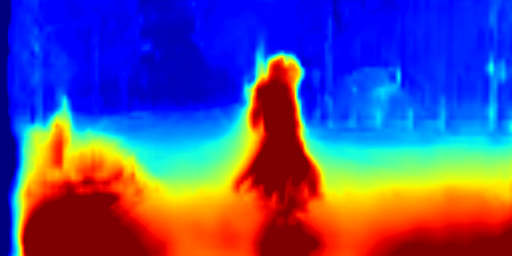
\includegraphics[width=0.19\linewidth]{image_000050_000019_depth.png}
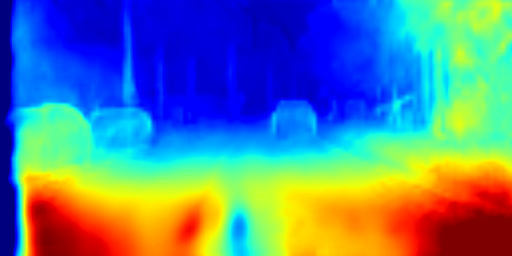
\includegraphics[width=0.19\linewidth]{image_000045_000019_depth.png}
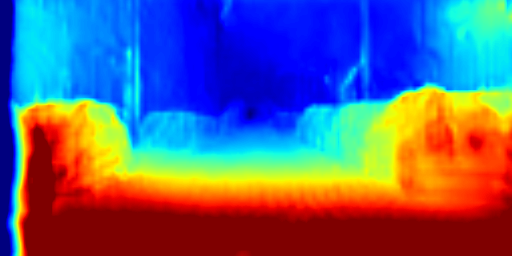
\includegraphics[width=0.19\linewidth]{image_000046_000019_depth.png}
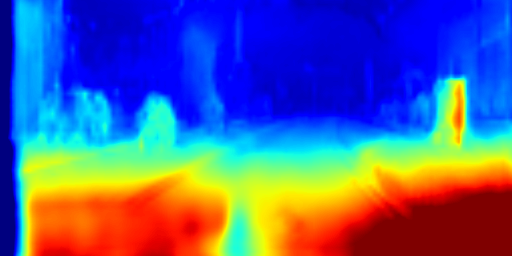
\includegraphics[width=0.19\linewidth]{image_000038_000019_depth.png}
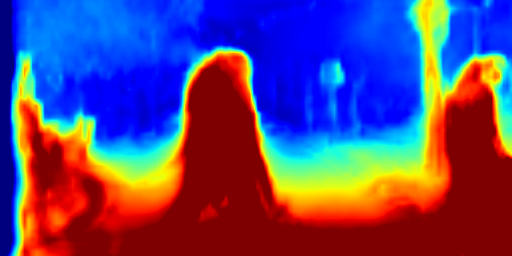
\includegraphics[width=0.19\linewidth]{image_000071_000019_depth.png}
\vspace{-2mm}
  \caption{Depth estimation}
\end{center}
\end{subfigure}

\begin{subfigure}[t]{\linewidth}
\begin{center}
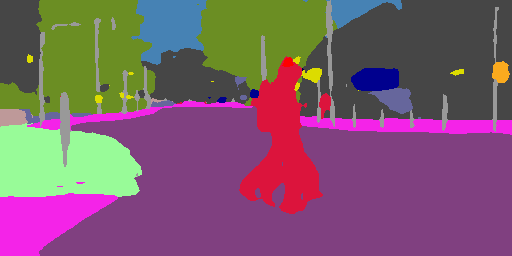
\includegraphics[width=0.19\linewidth]{image_000050_000019_segmentation.png}
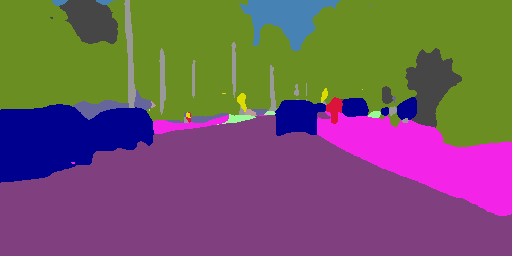
\includegraphics[width=0.19\linewidth]{image_000045_000019_segmentation.png}
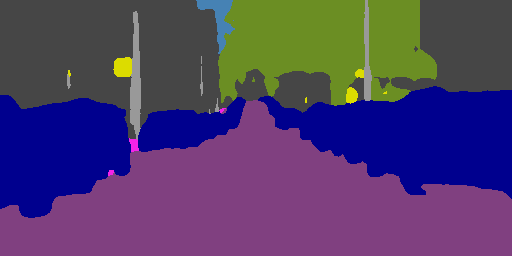
\includegraphics[width=0.19\linewidth]{image_000046_000019_segmentation.png}
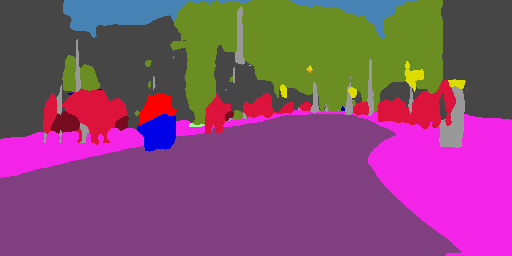
\includegraphics[width=0.19\linewidth]{image_000038_000019_segmentation.png}
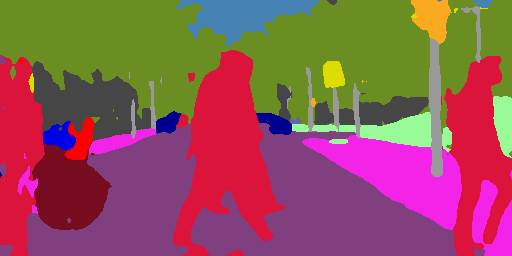
\includegraphics[width=0.19\linewidth]{image_000071_000019_segmentation.png}
\vspace{-2mm}
  \caption{Semantic segmentation}
\end{center}
\end{subfigure}
\vspace{-2mm}
   \caption[Qualitative results on CityScapes.]{\textbf{Qualitative results} for video scene understanding using our model. We observe good performance at semantic segmentation, optical flow, ego-motion and depth estimation. Examples are shown from validation sequences.}
\label{fig:results}
\vspace{-3mm}
\end{figure*}


We describe three main challenges for training video scene understanding models, which have largely prevented prior models achieving superior performance to date. We discuss three tricks which address these challenges which we show are critical to achieving good performance when training video scene understanding models.

\subsection{Trick \#1: Account for Motion when Propagating States.} 

In \sct{model} we presented the hypothesis that naive temporal convolutional models using recurrent units (e.g. \cite{patraucean2015spatio,valipour2017recurrent}) degraded performance compared to equivalent per-frame models, because they are unable to account for motion. In this section, we show that our motion-GRU improves performance over a per-frame baseline. We use self-supervised learning with photometric reprojection error to learn a representation of optical flow.

We also found that it was beneficial to initialise the recurrent connections such that they are close to identity connections \cite{he2016deep}, similar to the work of \cite{gadde2017semantic}. To achieve this, we offset the bias in the motion-GRU gates to $4.0$ so that the initialisation of the sigmoid function evaluates to near $1.0$. Consequently, the state will be almost entirely forgotten, and the signal almost entirely propagated from the current time-step. The model incrementally learns to incorporate temporal information by back-propagation.

\tbl{motion} confirms that adding a standard GRU degrades both segmentation accuracy and temporal consistency, compared to a per-frame baseline. This experiment also shows a significant improvement in performance when using our motion-GRU. This suggests that the motion-GRU is able to effectively propagate information temporally, by aligning features and accounting for dynamic scene motion.
In addition, our temporal consistency loss further improves performance by explicitly enforcing temporal consistency during training.

\begin{table}[t]
\begin{center}
	\begin{tabular}{l|c|c|c|c}
    \hline
    & \multicolumn{2}{c|}{Segmentation} & Depth & Flow \\
    Recurrent Model & IoU & Consistency & Err. ($px$) & Err. ($px$) \\
    \hline\hline
    per-frame baseline (no motion) & 63.9\% & 82.3\% & 11.2 & - \\
    GRU & 63.5\% & 87.4\% & 9.3 & 14.7 \\
    motion-GRU & 65.6\% & 91.9\% & \textbf{9.1} & 12.3 \\
    motion-GRU + consistency loss & \textbf{65.9\%} & \textbf{94.2\%} & 9.4 & \textbf{12.1} \\
    \hline
	\end{tabular}
\end{center}
\vspace{-2mm}
\caption[Importance of modelling motion.]{\textbf{Importance of modelling motion.} We compare our motion-GRU to baseline models and quantify the improvement due to modelling motion and increasing sequence length. Naively adding recurrent units to a segmentation model degrades performance. The motion-aware recurrent architecture improves performance. Our temporal consistency loss improves results further.}
\label{tbl:motion}
\vspace{-5mm}
\end{table}

\subsection{Trick \#2: Learn Stable Representations with Temporal Data Augmentation.}

In order to train effective video models with good temporal consistency, it is important to train over long video sequences. It is essential to have a number of frames so that the model can learn higher order dynamics and motion. Previous work only considers training over small sequences, often with only two frames \cite{gadde2017semantic}, which makes it impossible for the model to learn higher-order motion.

However, we find two problems when attempting to train on long video sequences: (1) training over a fixed sequence length results in an unstable model, and (2) we cannot back-propagate through long sequences given our available GPU memory. To overcome these problems, we use \textit{temporal data augmentation}.

To explain the first problem, let us consider training a model using sequences of fixed length $N$, with only the frame at $t=N$ labelled. We observe the model learns to develop a representation which is able to make a prediction very effectively at time $t=N$. However, leading up to this time, and beyond if we run the recurrent model continuously, the state becomes unstable and diverges. Our intuition is this is because the model has not been taught to make predictions continuously, it is only optimised to predict at time $t=N$. Therefore to address this issue, we propose to randomly vary the sequence length during training, and the position of the labelled frame, which we term \textit{temporal data augmentation}.

Regarding the second issue, back-propagating gradients over video requires significant amounts of GPU memory as feature representations from previous time-steps must be retained in memory. To overcome this, we propose to forward propagate over long (potentially infinite) video sequences, but only back-propagate over a shorter fixed time horizon. We refer to the forward-only data as a \textit{warm-up} as it produces a recurrent state which is used to train over the remaining sequence data. This reduces GPU memory requirements as we can discard feature activations from memory for all time-steps during the warm-up phase. Our final approach is to train using a different random warm-up length for each mini-batch during training.

In \tbl{timesteps}, we compare the effect of training over different length time-steps. We observe an improvement with training over longer time sequences, including with a random warm-up when the sequence is too long to back-propagate in memory.

\begin{table}[t]
\begin{center}
	\begin{tabular}{l|c|c|c|c}
    \hline
    & \multicolumn{2}{c|}{Segmentation} & Depth & Flow \\
    Time-steps & IoU & Consistency & Err. ($px$) & Err. ($px$) \\
		\hline\hline
         1 & 63.9\% & 82.3\% & 11.2 & - \\
		2 & 64.6\% & 89.1\% & 9.8 & 14.5 \\
		4 & 65.9\% & 92.3\% & 9.5 & 12.7 \\
		4 + 4 random warm-up &  \textbf{65.9\%} & \textbf{94.2\%} & \textbf{9.4} & \textbf{12.1} \\
		\hline
	\end{tabular}
\end{center}
\vspace{-2mm}
\caption[Method and sequence used for training video models.]{\textbf{Method and sequence used for training video models} has a massive impact on model performance. We observe training over longer sequences improves performance. In addition to improving performance, we also find that randomly varying training sequence length forces the model to learn a temporally stable representation, allowing the model to be run recurrently for indefinite time-sequences.}
\label{tbl:timesteps}
\vspace{-5mm}
\end{table}

\begin{table}[t]
\begin{center}
	\begin{tabular}{l|c|c|c|c|c}
    \hline
    & \multicolumn{2}{c|}{Segmentation} & Depth & Flow & Egomotion\\
    Tasks & IoU & Consistency & Err. ($px$) & Err. ($px$)& Err. ($m$) \\
    \hline\hline
    segmentation & 63.8\% & 82.7\% & - & - & - \\
    segmentation+flow & 65.1\% &91.3\% & - & 14.1 & - \\
    segmentation+flow+mono depth & 65.6\% & 93.8\% & 21.8** & 12.3 & 0.39** \\
    segmentation+flow+stereo depth & \textbf{65.9\%} & \textbf{94.2\%} & \textbf{9.4} & \textbf{12.1} & - \\
    \hline
	\end{tabular}
\end{center}
\vspace{-2mm}
\caption[Benefit of self-supervised and multi-task learning.]{\textbf{Benefit of self-supervised and multi-task learning.} These experiments illustrate the improvement our approach receives from multi-task learning. Learning representations of motion and geometry significantly improves performance of semantic segmentation. **We can only resolve the monocular depth and ego-motion prediction up to some scale-ambiguity. To compute accuracy, we optimise the scale factor using the validation data.}
\label{tbl:multitask}
\vspace{-5mm}
\end{table}

\begin{figure*}[t]
\begin{tabularx}{\textwidth}{@{}YYYYY@{}}
\hline
$\mathbf{t-10}$ & $\mathbf{t-5}$ & $\mathbf{t-3}$ & $\mathbf{t-2}$ & $\mathbf{t}$ \\
\hline
\end{tabularx}

\begin{subfigure}[t]{\linewidth}
\begin{center}
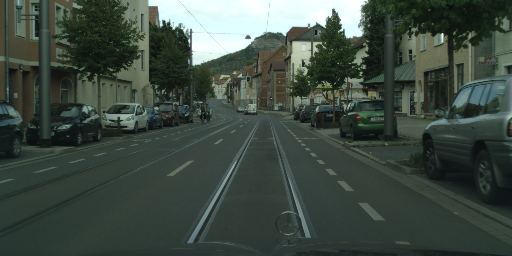
\includegraphics[width=0.19\linewidth]{seq/image_000086_000001_image.png}
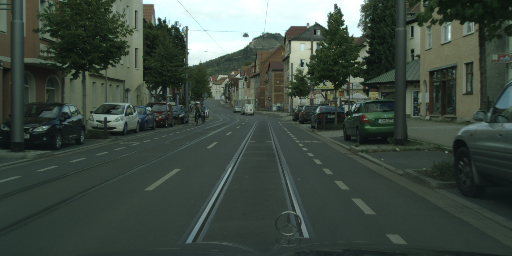
\includegraphics[width=0.19\linewidth]{seq/image_000086_000004_image.png}
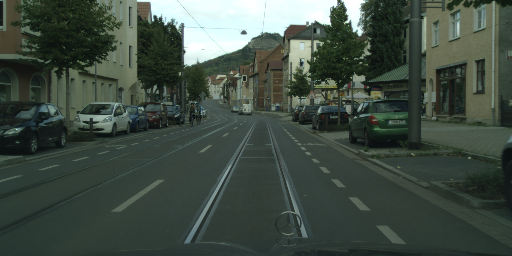
\includegraphics[width=0.19\linewidth]{seq/image_000086_000007_image.png}
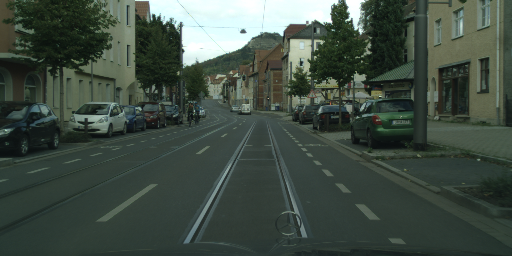
\includegraphics[width=0.19\linewidth]{seq/image_000086_000008_image.png}
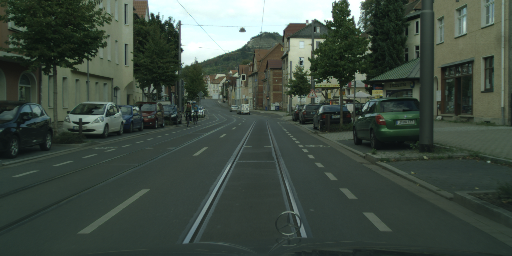
\includegraphics[width=0.19\linewidth]{seq/image_000086_000009_image.png}
\vspace{-2mm}
  \caption{Input video sequence}
\end{center}
\end{subfigure}

%\begin{subfigure}[t]{\linewidth}
%\begin{center}
%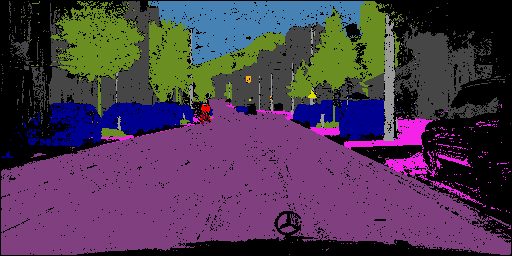
\includegraphics[width=0.195\linewidth]{seq/image_000086_000001_label.png}
%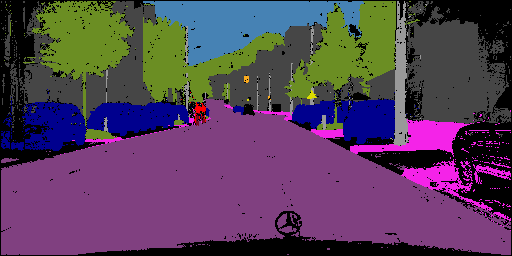
\includegraphics[width=0.19\linewidth]{seq/image_000086_000004_label.png}
%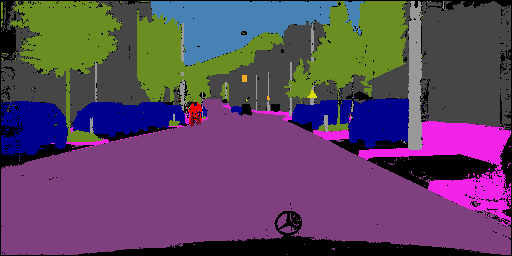
\includegraphics[width=0.19\linewidth]{seq/image_000086_000007_label.png}
%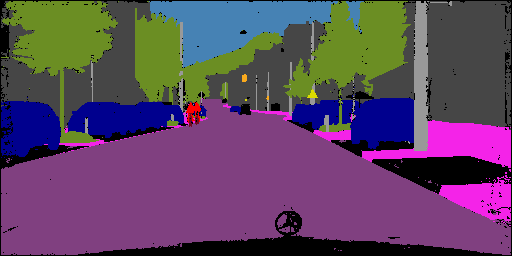
\includegraphics[width=0.19\linewidth]{seq/image_000086_000008_label.png}
%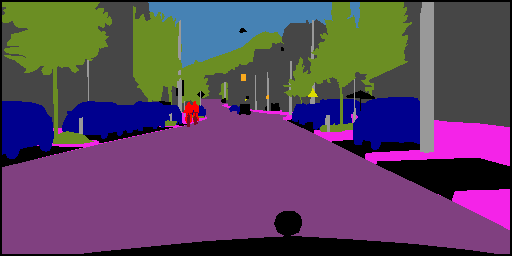
\includegraphics[width=0.19\linewidth]{seq/image_000086_000009_label.png}
%  \caption{Semantic Segmentation labels \cite{Cordts2016Cityscapes} and propagated by \cite{budvytis2017large,budvytis2010label}}
%\end{center}
%\end{subfigure}

\begin{subfigure}[t]{\linewidth}
\begin{center}
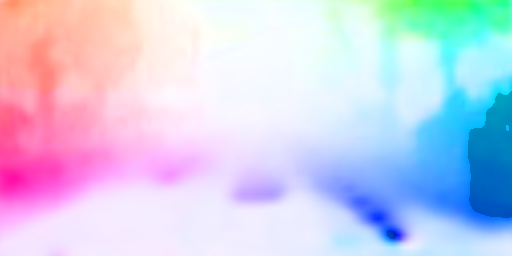
\includegraphics[width=0.19\linewidth]{seq/image_000086_000001_flow.png}
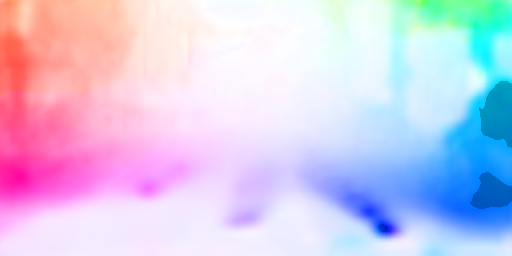
\includegraphics[width=0.19\linewidth]{seq/image_000086_000004_flow.png}
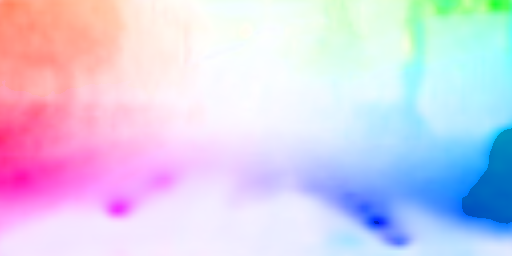
\includegraphics[width=0.19\linewidth]{seq/image_000086_000007_flow.png}
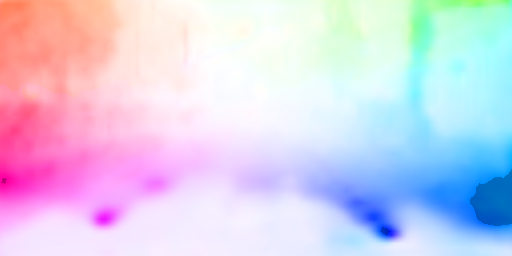
\includegraphics[width=0.19\linewidth]{seq/image_000086_000008_flow.png}
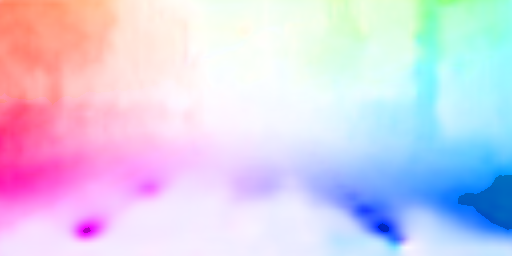
\includegraphics[width=0.19\linewidth]{seq/image_000086_000009_flow.png}
\vspace{-2mm}
  \caption{Self-supervised optical flow estimation}
\end{center}
\end{subfigure}

\begin{subfigure}[t]{\linewidth}
\begin{center}
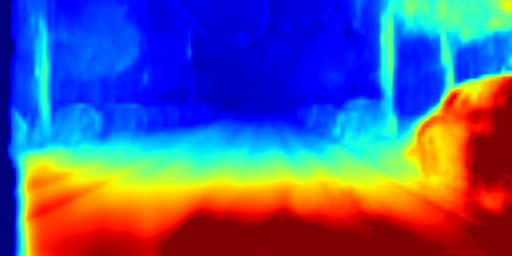
\includegraphics[width=0.19\linewidth]{seq/image_000086_000001_depth.png}
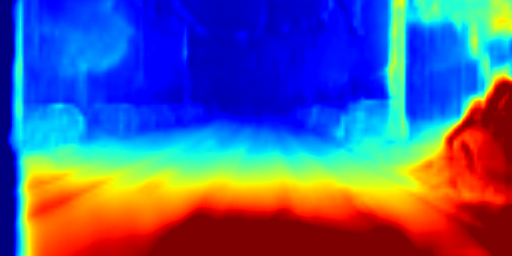
\includegraphics[width=0.19\linewidth]{seq/image_000086_000004_depth.png}
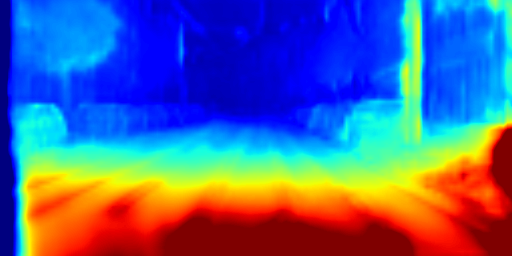
\includegraphics[width=0.19\linewidth]{seq/image_000086_000007_depth.png}
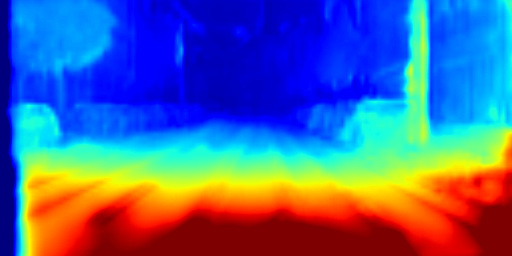
\includegraphics[width=0.19\linewidth]{seq/image_000086_000008_depth.png}
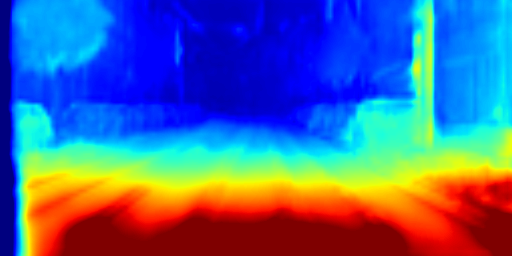
\includegraphics[width=0.19\linewidth]{seq/image_000086_000009_depth.png}
\vspace{-2mm}
  \caption{Self-supervised video depth estimation.}
\end{center}
\end{subfigure}

\begin{subfigure}[t]{\linewidth}
\begin{center}
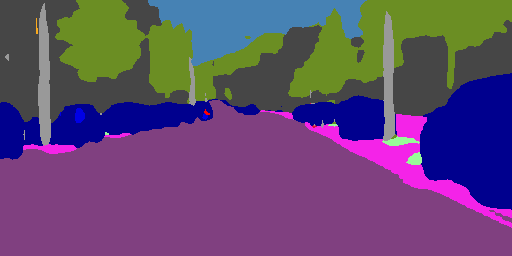
\includegraphics[width=0.19\linewidth]{seq/image_000086_000001_segmentation.png}
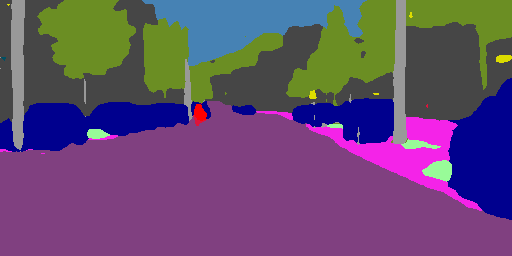
\includegraphics[width=0.19\linewidth]{seq/image_000086_000004_segmentation.png}
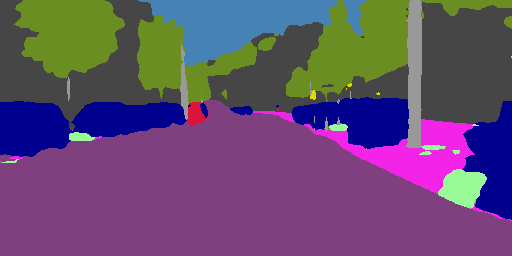
\includegraphics[width=0.19\linewidth]{seq/image_000086_000007_segmentation.png}
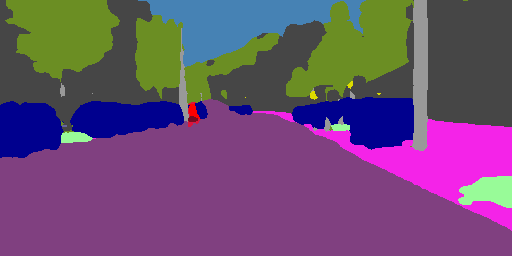
\includegraphics[width=0.19\linewidth]{seq/image_000086_000008_segmentation.png}
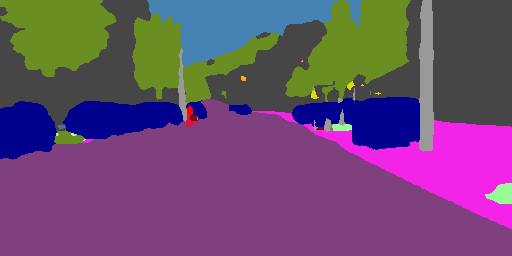
\includegraphics[width=0.19\linewidth]{seq/image_000086_000009_segmentation.png}
\vspace{-2mm}
  \caption{Video semantic segmentation.}
\end{center}
\end{subfigure}
\vspace{-2mm}
   \caption[Video sequence results.]{\textbf{Video semantic segmentation over a 10 frame sequence.} We observe that by learning motion and geometry and leveraging motion cues over video results in temporally consistent segmentation with less flickering between classes in the video output. We observe an increased ability to learn thin structures and difficult classes compared to the baseline.}
\label{fig:results2}
\vspace{-3mm}
\end{figure*}


\subsection{Trick \#3: Provide a Dense Loss at Each Time-Step.} 

%Typically, not every frame has dense pixel-wise semantic labels, as they are expensive to label. While we can learn geometry and motion across all frames using self-supervised learning, this makes it hard to learn temporally consistent semantic segmentation maps. To address this, we propose to use label propagation \cite{budvytis2010label} to augment sparely labelled frames over time. This is an off-line process, taking weeks to propagate large amounts of data with graphical models \cite{budvytis2010label}. We use the dataset from \cite{budvytis2017large}, who provide propagated labels in the CityScapes dataset \cite{Cordts2016Cityscapes}, for 10 frames forward and backward from each labelled frame.

Finally, we find that it is important to provide a rich training signal over large amounts of data to learn video scene understanding models. However, labelling frames densely in video is prohibitively expensive. Therefore our third trick is to utilise self-supervised learning to provide a training signal for each frame.

We learn optical flow using self-supervised learning with the loss in \eqn{flow}. We show results for training depth using stereo reprojection error with the loss given by \eqn{depth}. However, since this requires stereo data, we also show results using the loss in \eqn{monodepth} to learn depth and ego-motion using monocular temporal reprojection. For all models, we use the probabilistic multi-task loss from \cite{kendall2017multi} to balance the individual task losses.

In \tbl{multitask} we train models with different combinations of task losses, over a sequence of four frames and a warm-up of four frames. We observe a large quantitative improvement in results by modelling geometry. Learning with motion and depth features significantly improves performance further. Providing stereo data marginally outperforms monocular depth supervision. However, the monocular depth and ego-motion model is competitive, if only monocular data is available for training. 

\fig{results} shows qualitative performance. The self-supervised learning produces smooth and robust estimates of geometry, and the model is noticeably more temporally consistent than the per-frame E-Net baseline. \fig{results2} shows a single 10-frame sequence.

%\subsection{Efficiency.}
%On a single NVIDIA Titan Xp GPU, our model takes $160$ milliseconds per-frame for inference of $1024 \times 512$ images. This framework adds a relatively small computational cost over single-frame semantic segmentation models. Unlike NetWarp \cite{gadde2017semantic}, we do not need to re-encode the previous image to learn motion. Rather, our model can propagate state with recurrent connections.

\section{Conclusions}

In this chapter, we investigated the problem of video scene understanding. We briefly summarise the main conclusions within the three main themes of this dissertation.

\textbf{End-to-end deep learning.}
In this chapter, we have demonstrated an end-to-end deep learning model to learn semantic segmentation, optical flow and scene depth from video sequences in real-time. We show how to design recurrent units which can compensate for ego-motion and align features over time. Through a number of experiments, we present insights for training temporal models to form temporally consistent representations from long video sequences. We find that end-to-end learning over long video sequences outperforms models trained on individual frames.

\textbf{Geometry.}
We show that explicitly modelling geometry, in the form of depth and motion, is critical to obtain accurate feature representations over video sequences. We demonstrate how to use geometry to align features over time, improving segmentation performance. This allows us to improve on the per-frame segmentation model by leveraging motion features. Jointly representing depth, in addition to semantics, further improves model performance.

We find that in order to train over long video sequences, it is important to provide a training signal for each frame. Labelling the semantics of each frame is too expensive. Therefore we demonstrate that learning motion and depth with unsupervised learning is an effective method to provide a training signal for each image in a long video sequence.

\textbf{Uncertainty.}
While the probabilistic techniques from the previous chapters can be applied to this model, this chapter does not explicitly explore the application of uncertainty to the problem of video scene understanding. However, we utilise uncertainty for multi-task learning using the technique from \cref{sec:multitask} to simultaneously learn depth, motion and semantics.

